\documentclass{beamer}

\usepackage{listings}
\usepackage{slashbox}
\usepackage{tikz}
\usepackage{booktabs}
\usepackage{amsmath,amssymb}
\usepackage{hyperref}
\usepackage{graphicx}

\DeclareMathOperator*{\argmin}{arg\,min}
\DeclareMathOperator*{\argmax}{arg\,max}
\DeclareMathOperator*{\maximize}{maximize}
\DeclareMathOperator*{\minimize}{minimize}
\newcommand{\sign}{\operatorname{sign}}
\newcommand{\RR}{\mathbb R}
\newcommand{\NN}{\mathbb N}

% Set transparency of non-highlighted sections in the table of
% contents slide.
\setbeamertemplate{section in toc shaded}[default][100]
\AtBeginSection[]
{
  \setbeamercolor{section in toc}{fg=red} 
  \setbeamercolor{section in toc shaded}{fg=black} 
  \begin{frame}
    \tableofcontents[currentsection]
  \end{frame}
}

\begin{document}

\title{Support vector comparison machines}
\author{
Toby Dylan Hocking\\
toby.hocking@mail.mcgill.ca\\
joint work with David Venuto,  Lakjaree Sphanurattana, and Masashi Sugiyama
}

\date{2 March 2018}

\maketitle

\section{Introduction and related work}

\begin{frame}
  \frametitle{Motivating example: learning to compare sushi}
  \includegraphics[width=1in]{sushi_salmon}\makebox[2.5in]{salmon is
    better than eel}\includegraphics[width=1in]{sushi_anago}

  \includegraphics[width=1in]{sushi_chu-toro}\makebox[2.5in]{\alert<2>{fatty
      tuna is as good as
      crab liver}}\includegraphics[width=1in]{sushi_kani-miso}

If I give you another sushi pair,\\
can you tell me which one is better,\\
\alert<2>{or if they are equally good?}
\end{frame}

\begin{frame}
  \frametitle{Learning a comparison function}
  We are given $n$ training pairs $(\mathbf x_i,\mathbf x_i',y_i)$ 
  \begin{itemize}
  \item Input: a pair of feature vectors $\mathbf x_i,\mathbf x_i'\in\RR^p$\\
    e.g. sushi fattiness, taster birthplace.
  \item Output: a label $y_i=
  \begin{cases}
    -1 & \text{ if $\mathbf x_i$ is better}\\
    0 & \text{ if $\mathbf x_i$ is as good as $\mathbf x'_i$}\\
    1 & \text{ if $\mathbf x'_i$ is better}.
  \end{cases}
$
  \end{itemize}
  Goal: find a comparison function
  $c:\RR^p\times\RR^p\rightarrow\{-1,0,1\}$
\begin{itemize}
\item Good prediction with respect to the zero-one loss:
$$\minimize_c \sum_{i\in\text{test}} 
I\left[ y_i \neq c(\mathbf x_i,\mathbf x_i') \right]$$
\item Symmetry: $c(\mathbf x,\mathbf x') = -c(\mathbf x',\mathbf x)$.
\end{itemize}
\end{frame}

\begin{frame}
  \frametitle{Geometric interpretation when $r(\mathbf x)=||\mathbf
    x||_2^2$}
  \begin{minipage}{1.0\linewidth}
    \hskip -0.5cm
      \input{figure-geometry}
  \end{minipage}
\end{frame}

\begin{frame}
  \frametitle{Geometric interpretation when $r(\mathbf x)=||\mathbf
    x||_2^2$}
  \begin{minipage}{1.0\linewidth}
    \hskip -0.5cm
  \input{figure-norm-data}
  \end{minipage}
\end{frame}

\begin{frame}
  \frametitle{Related work: rank and rate}
\renewcommand{\arraystretch}{1.5}
\begin{tabular}{|c|c|c|}\hline
  \backslashbox{Outputs}{Inputs}
  &single items $\mathbf x$&pairs of items $\mathbf x,\mathbf x'$\\ \hline
  $y\in\{-1,1\}$ &SVM  & SVMrank   	\\ \hline 
  $y\in\{-1,0,1\}$ && this work\\ \hline
\end{tabular}
\begin{itemize}
\item T Joachims. Optimizing search engines using clickthrough
  data. KDD 2002. (SVMrank)
\item K Zhou \emph{et al.} Learning to rank with ties. SIGIR
  2008. (boosting, ties are more effective with more output values)
\item R Herbrich \emph{et al.} TrueSkill: a Bayesian skill rating
  system. NIPS 2006. (generalization of Elo for chess)
\end{itemize}
\end{frame}

\begin{frame}
  \frametitle{SVMrank ignores equality $y_i=0$ pairs}
  Linear $r(\mathbf x) = \mathbf w^\intercal \mathbf x$.
  \begin{equation*}
    \begin{aligned}
          \minimize_{\mathbf w\in\RR^p}\ \  & \mathbf w^\intercal \mathbf w \\
          \text{subject to}\ \  & 
          \mathbf w^\intercal(\mathbf x_i'-\mathbf x_i)y_i \geq 1,
          \ \forall i\text{ such that }y_i\in\{-1,1\}.
    \end{aligned}
  \end{equation*}
  \input{figure-max-margin-bothsides-svmrank}
\end{frame}

\section{Learning a max-margin comparison function}

\begin{frame}
  \frametitle{Learning to rank and compare}
  We will learn a
  \begin{itemize}
  \item Ranking function $r:\RR^p\rightarrow\RR$. Bigger is better.
  \item Threshold $\tau\in\RR^+$. \\A small difference
    $|r(\mathbf x')-r(\mathbf x)|\leq \tau$ is not significant.
  \item Comparison function $c_\tau(\mathbf x, \mathbf x') =
  \begin{cases}
    -1 & \text{ if }r(\mathbf x')-r(\mathbf x) < -\tau\\
    0 & \text{ if }|r(\mathbf x')-r(\mathbf x)|\leq \tau\\
    1 & \text{ if }r(\mathbf x')-r(\mathbf x) > \tau.
  \end{cases}
$
\end{itemize}
Fix the threshold $\tau=1$. The problem becomes
$$\minimize_{r} \sum_{i=1}^n 
I\left[ y_i\neq c_1(\mathbf x_i, \mathbf x_i') \right].$$
If there are several $r$ that achieve 0 error, \\
then the data are separable.
\end{frame}

\begin{frame}
  \frametitle{Max margin LP for separable data}
  \underline{Linear Program (LP) measures ranking function values:}
  \begin{equation*}
  \begin{aligned}
    \maximize_{\mu\in\RR, \mathbf w\in\RR^p}\ & \mu \\
    \text{subject to}\ & 
    \mu \leq 1-|\mathbf w^\intercal (\mathbf x_i' - \mathbf x_i)|,\
    \forall\  i\text{ such that }y_i=0,\\
    &\mu \leq -1 +  
    \mathbf w^\intercal(\mathbf x_i'-\mathbf x_i)y_i,
    \ \forall\ i\text{ such that }y_i\in\{-1,1\}.
  \end{aligned}
\end{equation*}
\begin{itemize}
\item If the optimal margin $\mu>0$ then the data are separable.
\item Ranking function $r(\mathbf x) = \mathbf w^\intercal \mathbf x$.
\item Comparison function $c_1(\mathbf x, \mathbf x')$.
\end{itemize}
\end{frame}

\begin{frame}
  \frametitle{Geometric interpretation of max margin LP}
  \input{figure-hard-margin-one}
\end{frame}

\begin{frame}
  \frametitle{Equivalent: $(\mathbf x_i, \mathbf x_i', y_i=-1)$ flipped to $(\mathbf x_i', \mathbf x_i, \tilde y_i=1)$}
  \input{figure-hard-margin-flipneg}
\end{frame}

\begin{frame}
  \frametitle{Max margin SVM QP for separable data}
  \underline{Change of variables \alert<2>{``flipped data''}}
  \begin{equation*}
\label{eq:tilde}
\mathbf{  \tilde X} = \left[
    \begin{array}{c}
      \mathbf X_1 \\
      \alert<2>{\mathbf X_{-1}'}\\
      \mathbf X_0\\
      \alert<2>{\mathbf X_0'}
    \end{array}
  \right],\ 
  \mathbf{\tilde X'} = \left[
    \begin{array}{c}
      \mathbf X_1' \\
      \alert<2>{\mathbf X_{-1}}\\
      \mathbf X_0'\\
      \alert<2>{\mathbf X_0}
    \end{array}
  \right],\ 
  \mathbf{\tilde y} = \left[
    \begin{array}{c}
      \mathbf 1_{|\mathcal I_1|} \\
      \alert<2>{\mathbf 1_{|\mathcal I_{-1}|}}\\
      \mathbf{-1}_{|\mathcal I_0|}\\
      \alert<2>{\mathbf{-1}_{|\mathcal I_0|}}
    \end{array}
  \right],
\end{equation*}
\vskip -0.5cm
\begin{itemize}
\item  $\tilde y_i=-1$ implies no significant
difference between $\mathbf{\tilde x}_i$ and $\mathbf{\tilde x}_i'$,
\item  $\tilde y_i=1$ implies that $\mathbf{\tilde x}_i'$ is better than
$\mathbf{\tilde x}_i$.
\end{itemize}
  \underline{Quadratic Program measures weight vector size (SVM QP)}
\begin{eqnarray*}
  \label{eq:max-margin-qp-tilde}
  \minimize_{\mathbf u\in\RR^p, \beta\in\RR}\ &&\hskip -0.5cm
  \mathbf u^\intercal \mathbf u  \\
\nonumber    \text{subject to}\ &&\hskip -0.5cm 
    \tilde y_i (\beta + 
    \mathbf u^\intercal( \mathbf{\tilde x}_i'-\mathbf{\tilde x}_i) ) \geq 1,
    \ \forall i\in\{1,\dots,m\}.
\end{eqnarray*}
Same as SVM: learn affine function $f(\mathbf x)=\beta+\mathbf
u^\intercal \mathbf x$.\\
\textbf{Lemma:} $\hat{\mu} = -1/\beta$,
$\hat{ \mathbf{w}} = -\mathbf{u}/\beta$ are feasible for the LP.
\end{frame}

\begin{frame}
  \frametitle{Equivalent: $(\mathbf x_i, \mathbf x_i', y_i=-1)$ flipped to $(\mathbf x_i', \mathbf x_i, \tilde y_i=1)$}
  \input{figure-hard-margin-flipneg}
\end{frame}

\begin{frame}
  \frametitle{QP sensitive to feature scale}
  \input{figure-hard-margin-flipneg-qp}
\end{frame}

\begin{frame}
  \frametitle{$(\mathbf x_i, \mathbf x_i', y_i=0)$ flipped to
    $(\mathbf x_i, \mathbf x_i', \tilde y_i=-1)$
}
  \input{figure-hard-margin-flipneg.scaled-qp}
\end{frame}

\begin{frame}
  \frametitle{$(\mathbf x_i, \mathbf x_i', y_i=0)$ flipped to
    $(\mathbf x_i, \mathbf x_i', \tilde y_i=-1)$,
    $(\mathbf x_i', \mathbf x_i, \tilde y_i=-1)$
}
  \input{figure-hard-margin-both.scaled-qp}
\end{frame}

\begin{frame}
  \frametitle{Max margin LP and QP for separable data}
  \underline{Linear Program (LP) measures function values:}
  \begin{equation*}
  \begin{aligned}
    \maximize_{\mu\in\RR, \mathbf w\in\RR^p}\ & \mu \\
    \text{subject to}\ & 
    \mu \leq 1-|\mathbf w^\intercal (\mathbf x_i' - \mathbf x_i)|,\
    \forall\  i\text{ such that }y_i=0,\\
    &\mu \leq -1 +  
    \mathbf w^\intercal(\mathbf x_i'-\mathbf x_i)y_i,
    \ \forall\ i\text{ such that }y_i\in\{-1,1\}.
  \end{aligned}
\end{equation*}
\vskip 0.5cm
  \underline{Quadratic Program (QP) measures weight vector size:}
\begin{eqnarray*}
  \label{eq:max-margin-qp-tilde}
  \minimize_{\mathbf u\in\RR^p, \beta\in\RR}\ &&\hskip -0.5cm
  \mathbf u^\intercal \mathbf u  \\
\nonumber    \text{subject to}\ &&\hskip -0.5cm 
    \tilde y_i (\beta + 
    \mathbf u^\intercal( \mathbf{\tilde x}_i'-\mathbf{\tilde x}_i) ) \geq 1,
    \ \forall i\in\{1,\dots,m\}.
\end{eqnarray*}
\begin{itemize}
\item 
\textbf{Lemma:} $\hat{\mu} = -1/\beta$, $\hat{ \mathbf{w}} =
-\mathbf{u}/\beta$ are feasible for the LP.\\
\item Ranking functions
  $r_{\text{LP}}(\mathbf x) = \mathbf w^\intercal \mathbf x$,
  $r_{\text{QP}}(\mathbf x) = \hat{\mathbf w}^\intercal \mathbf x$.
\item Comparison function $c_1(\mathbf x, \mathbf x')$.
\end{itemize}
\end{frame}

\section{Results and conclusions}

\begin{frame}
  \frametitle{Simulation: true patterns $r$ and noisy training pairs}
  \begin{minipage}{1.0\linewidth}
    \hskip -0.5cm \input{figure-truth-train} Validation and test data
    have the same number of pairs $n$ and the same proportion of
    equality pairs $\rho$.
  \end{minipage}
\end{frame}

\begin{frame}
  \frametitle{Details of simulation setup}
  \begin{itemize}
    \item Inputs $\mathbf x_i,\mathbf x_i'\in[-3,3]^2$.
    \item True ranking function $r(\mathbf x)=||\mathbf x||^2_j$ 
      for $j\in\{1,2,\infty\}$.
    \item Noisy labels $y_i=t_1[r(\mathbf x'_i)-r(\mathbf x_i)+\epsilon_i]$.
  \item Threshold function
$
  \label{eq:threshold}
  t_1(x) = 
  \begin{cases}
    -1 & \text{ if } x < -1, \\
    0 & \text{ if } |x| \leq 1, \\
    1 & \text{ if } x > 1. \\
  \end{cases}
$
\item Noise $\epsilon_i\sim N(0, \sigma)$ with standard deviation
  $\sigma=1/4$.
\item Train, validation, and test sets with
  \begin{itemize}
    \item same number of training pairs $n$, and
    \item same proportion of equality pairs $\rho$.
  \end{itemize}
\item Fit a $10\times 10$ grid of models to the training
set:
\begin{itemize}
\item Cost parameter $C=10^{-3},\dots,10^3$,
\item Gaussian kernel width $2^{-7},\dots,2^4$.
\end{itemize}
\item Select the model with minimal zero-one loss on the validation set.
  \end{itemize}
\end{frame}

\begin{frame}
  \frametitle{We ran 3 different algorithms on each data set}
  \begin{center}
        \begin{tabular}{r|cc|cc|c|}
&    \multicolumn{2}{c|}{equality pairs}
&    \multicolumn{2}{c|}{inequality pairs}\\
Input:    & $|\mathcal I_0|$ %$\tilde y_i= -1$
    & --- 
    & $|\mathcal I_1|+|\mathcal I_{-1}|$ %$\tilde y_i=1$
    & $\rightarrow$ &
    code
    \\
    \hline
    rank 
    & 0 
    & 
    & $|\mathcal I_1|+|\mathcal I_{-1}|$ 
    & $\rightarrow$ &
    SVMrank
    \\
    \hline
    rank2 
    & $2|\mathcal I_0|$ 
    & $\leftarrow \rightarrow$
    & $2(|\mathcal I_1|+|\mathcal I_{-1}|)$ 
    & $\rightarrow \rightarrow$ &
    SVMrank
    \\
    \hline
    compare 
    & $2|\mathcal I_0|$ 
    & --- --- 
    & $|\mathcal I_1|+|\mathcal I_{-1}|$ 
    & $\rightarrow$ &
    proposed
    \\
    \hline
  \end{tabular}
  \end{center}
  \begin{description}
  \item[Equality $y_i=0$ pairs] are shown as ---  
    segments.
  \item[Inequality $y_i\in\{-1,1\}$ pairs]
    are shown as $\rightarrow$  arrows.
  \item[rank] ignores each input equality pair.
  \item[rank2] converts each input equality pair
    to two contradictory inequality pairs.
  \item[compare] directly models the equality pairs.
  \end{description}
\end{frame}

\input{sample-level-curves}

\begin{frame}
  \frametitle{Test error lowest for proposed SVMcompare model}
  \begin{minipage}{1.0\linewidth}
    \hskip -0.5cm
      \input{figure-simulation-samples-linf}
  \end{minipage}
\end{frame}

\begin{frame}
  \frametitle{Test error lowest for proposed SVMcompare model}
  \begin{minipage}{1.0\linewidth}
    \hskip -0.5cm
      \input{figure-simulation-samples}
  \end{minipage}
\end{frame}

\input{proportion-level-curves}

\begin{frame}
  \frametitle{No difference for few equality pairs,\\
    rank worse when there are many equality pairs}
  \begin{minipage}{1.0\linewidth}
    \hskip -0.5cm
      \input{figure-auc-linf}
  \end{minipage}
\end{frame}

\begin{frame}
  \frametitle{No difference for few equality pairs,\\
    rank worse when there are many equality pairs}
  \begin{minipage}{1.0\linewidth}
    \hskip -0.5cm
      \input{figure-auc}
  \end{minipage}
\end{frame}

\begin{frame}
  \frametitle{Sushi data of Kamishima et al.}
  \begin{itemize}
  \item  \url{http://www.kamishima.net/sushi/}
  \item 100 different sushis rated by 5000 different people.
  \item Each person rated 10 sushis on a 5 point scale. 
  \item Convert 10 ratings to 5 preference pairs.
  \item 17,832 equality $y_i=0$ pairs and
  \item 7,168 inequality $y_i\in\{-1,1\}$ pairs.
  \item Feature pairs $\mathbf x_i,\mathbf x_i'\in\RR^{14}$.
  \item 7 sushi features: style, major, minor, oily, eating frequency,
    price, and selling frequency.
  \item 7 taster/person features: Sushi gender, age, time, birthplace
    and current home (we converted Japanese prefecture codes to
    latitude/longitude coordinates).
  \end{itemize}
\end{frame}

\begin{frame}
  \frametitle{Sushi data are harder,\\
    but SVMcompare still has lowest test error}
  \begin{minipage}{1.0\linewidth}
    \hskip -1cm
      \input{figure-sushi}
  \end{minipage}
\end{frame}

\begin{frame}
  \frametitle{Chess data description}
  \begin{itemize}
  \item \url{http://www.chessmetrics.com}, 1999--2006 (eight years).
  \item For each year, train on first four months (Jan--Apr), test on
    other months (May--Dec).
  \item 44.7\% draws ($y_i=0$) -- predicting them is important!
  \item 16 features computed for each player and game: ELO score,
    Glicko score, initial move, loss/wins to a lower/higher ranked
    player, the average score difference of opponents,
    win/loss/draw/games played raw values and percentages, etc.
  \end{itemize}
\end{frame}

\begin{frame}
  \frametitle{Chess data result}
  \begin{minipage}{1.0\linewidth}
    \hskip -1cm
      % Created by tikzDevice version 0.10.1 on 2017-12-07 15:49:08
% !TEX encoding = UTF-8 Unicode
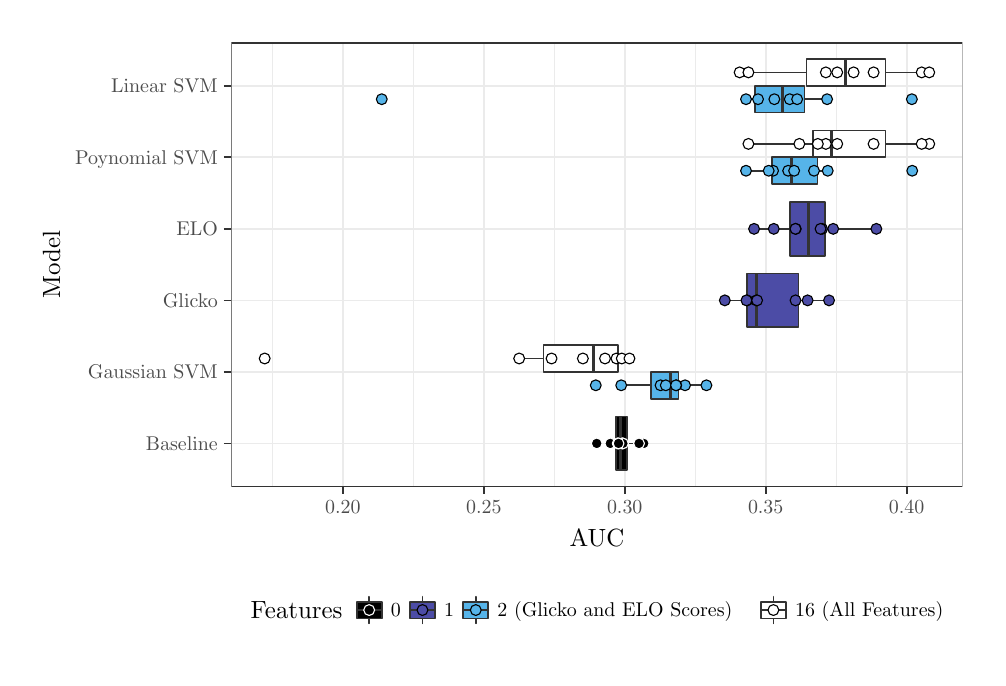
\begin{tikzpicture}[x=1pt,y=1pt]
\definecolor{fillColor}{RGB}{255,255,255}
\path[use as bounding box,fill=fillColor,fill opacity=0.00] (0,0) rectangle (343.28,227.65);
\begin{scope}
\path[clip] (  0.00,  0.00) rectangle (343.28,227.65);
\definecolor{drawColor}{RGB}{255,255,255}
\definecolor{fillColor}{RGB}{255,255,255}

\path[draw=drawColor,line width= 0.6pt,line join=round,line cap=round,fill=fillColor] (  0.00,  0.00) rectangle (343.28,227.65);
\end{scope}
\begin{scope}
\path[clip] ( 73.64, 61.91) rectangle (337.78,222.15);
\definecolor{fillColor}{RGB}{255,255,255}

\path[fill=fillColor] ( 73.64, 61.91) rectangle (337.78,222.15);
\definecolor{drawColor}{gray}{0.92}

\path[draw=drawColor,line width= 0.3pt,line join=round] ( 88.40, 61.91) --
	( 88.40,222.15);

\path[draw=drawColor,line width= 0.3pt,line join=round] (139.34, 61.91) --
	(139.34,222.15);

\path[draw=drawColor,line width= 0.3pt,line join=round] (190.28, 61.91) --
	(190.28,222.15);

\path[draw=drawColor,line width= 0.3pt,line join=round] (241.22, 61.91) --
	(241.22,222.15);

\path[draw=drawColor,line width= 0.3pt,line join=round] (292.16, 61.91) --
	(292.16,222.15);

\path[draw=drawColor,line width= 0.6pt,line join=round] ( 73.64, 77.42) --
	(337.78, 77.42);

\path[draw=drawColor,line width= 0.6pt,line join=round] ( 73.64,103.27) --
	(337.78,103.27);

\path[draw=drawColor,line width= 0.6pt,line join=round] ( 73.64,129.11) --
	(337.78,129.11);

\path[draw=drawColor,line width= 0.6pt,line join=round] ( 73.64,154.95) --
	(337.78,154.95);

\path[draw=drawColor,line width= 0.6pt,line join=round] ( 73.64,180.80) --
	(337.78,180.80);

\path[draw=drawColor,line width= 0.6pt,line join=round] ( 73.64,206.64) --
	(337.78,206.64);

\path[draw=drawColor,line width= 0.6pt,line join=round] (113.87, 61.91) --
	(113.87,222.15);

\path[draw=drawColor,line width= 0.6pt,line join=round] (164.81, 61.91) --
	(164.81,222.15);

\path[draw=drawColor,line width= 0.6pt,line join=round] (215.75, 61.91) --
	(215.75,222.15);

\path[draw=drawColor,line width= 0.6pt,line join=round] (266.69, 61.91) --
	(266.69,222.15);

\path[draw=drawColor,line width= 0.6pt,line join=round] (317.63, 61.91) --
	(317.63,222.15);
\definecolor{drawColor}{gray}{0.20}

\path[draw=drawColor,line width= 0.6pt,line join=round] (216.54, 77.42) -- (220.91, 77.42);

\path[draw=drawColor,line width= 0.6pt,line join=round] (212.54, 77.42) -- (210.53, 77.42);
\definecolor{fillColor}{RGB}{0,0,0}

\path[draw=drawColor,line width= 0.6pt,line join=round,line cap=round,fill=fillColor] (216.54, 67.73) --
	(212.54, 67.73) --
	(212.54, 87.11) --
	(216.54, 87.11) --
	(216.54, 67.73) --
	cycle;

\path[draw=drawColor,line width= 1.1pt,line join=round] (214.17, 67.73) -- (214.17, 87.11);

\path[draw=drawColor,line width= 0.6pt,line join=round] (235.17, 98.42) -- (245.27, 98.42);

\path[draw=drawColor,line width= 0.6pt,line join=round] (225.14, 98.42) -- (214.47, 98.42);
\definecolor{fillColor}{RGB}{86,180,233}

\path[draw=drawColor,line width= 0.6pt,line join=round,line cap=round,fill=fillColor] (235.17, 93.57) --
	(225.14, 93.57) --
	(225.14,103.27) --
	(235.17,103.27) --
	(235.17, 93.57) --
	cycle;

\path[draw=drawColor,line width= 1.1pt,line join=round] (232.42, 93.57) -- (232.42,103.27);

\path[draw=drawColor,line width= 0.6pt,line join=round] (213.24,108.11) -- (217.45,108.11);

\path[draw=drawColor,line width= 0.6pt,line join=round] (186.37,108.11) -- (177.60,108.11);
\definecolor{fillColor}{RGB}{255,255,255}

\path[draw=drawColor,line width= 0.6pt,line join=round,line cap=round,fill=fillColor] (213.24,103.27) --
	(186.37,103.27) --
	(186.37,112.96) --
	(213.24,112.96) --
	(213.24,103.27) --
	cycle;

\path[draw=drawColor,line width= 1.1pt,line join=round] (204.62,103.27) -- (204.62,112.96);

\path[draw=drawColor,line width= 0.6pt,line join=round] (278.55,129.11) -- (289.57,129.11);

\path[draw=drawColor,line width= 0.6pt,line join=round] (259.92,129.11) -- (251.91,129.11);
\definecolor{fillColor}{RGB}{76,76,166}

\path[draw=drawColor,line width= 0.6pt,line join=round,line cap=round,fill=fillColor] (278.55,119.42) --
	(259.92,119.42) --
	(259.92,138.80) --
	(278.55,138.80) --
	(278.55,119.42) --
	cycle;

\path[draw=drawColor,line width= 1.1pt,line join=round] (263.45,119.42) -- (263.45,138.80);

\path[draw=drawColor,line width= 0.6pt,line join=round] (288.07,154.95) -- (306.67,154.95);

\path[draw=drawColor,line width= 0.6pt,line join=round] (275.47,154.95) -- (262.48,154.95);

\path[draw=drawColor,line width= 0.6pt,line join=round,line cap=round,fill=fillColor] (288.07,145.26) --
	(275.47,145.26) --
	(275.47,164.65) --
	(288.07,164.65) --
	(288.07,145.26) --
	cycle;

\path[draw=drawColor,line width= 1.1pt,line join=round] (282.03,145.26) -- (282.03,164.65);

\path[draw=drawColor,line width= 0.6pt,line join=round] (285.39,175.95) -- (289.10,175.95);

\path[draw=drawColor,line width= 0.6pt,line join=round] (268.95,175.95) -- (259.57,175.95);
\definecolor{fillColor}{RGB}{86,180,233}

\path[draw=drawColor,line width= 0.6pt,line join=round,line cap=round,fill=fillColor] (285.39,171.11) --
	(268.95,171.11) --
	(268.95,180.80) --
	(285.39,180.80) --
	(285.39,171.11) --
	cycle;

\path[draw=drawColor,line width= 1.1pt,line join=round] (275.88,171.11) -- (275.88,180.80);

\path[draw=drawColor,line width= 0.6pt,line join=round] (310.01,185.65) -- (325.78,185.65);

\path[draw=drawColor,line width= 0.6pt,line join=round] (283.85,185.65) -- (260.44,185.65);
\definecolor{fillColor}{RGB}{255,255,255}

\path[draw=drawColor,line width= 0.6pt,line join=round,line cap=round,fill=fillColor] (310.01,180.80) --
	(283.85,180.80) --
	(283.85,190.49) --
	(310.01,190.49) --
	(310.01,180.80) --
	cycle;

\path[draw=drawColor,line width= 1.1pt,line join=round] (290.47,180.80) -- (290.47,190.49);

\path[draw=drawColor,line width= 0.6pt,line join=round] (280.75,201.80) -- (288.87,201.80);

\path[draw=drawColor,line width= 0.6pt,line join=round] (262.83,201.80) -- (259.57,201.80);
\definecolor{fillColor}{RGB}{86,180,233}

\path[draw=drawColor,line width= 0.6pt,line join=round,line cap=round,fill=fillColor] (280.75,196.95) --
	(262.83,196.95) --
	(262.83,206.64) --
	(280.75,206.64) --
	(280.75,196.95) --
	cycle;

\path[draw=drawColor,line width= 1.1pt,line join=round] (272.59,196.95) -- (272.59,206.64);

\path[draw=drawColor,line width= 0.6pt,line join=round] (310.01,211.49) -- (325.78,211.49);

\path[draw=drawColor,line width= 0.6pt,line join=round] (281.43,211.49) -- (257.26,211.49);
\definecolor{fillColor}{RGB}{255,255,255}

\path[draw=drawColor,line width= 0.6pt,line join=round,line cap=round,fill=fillColor] (310.01,206.64) --
	(281.43,206.64) --
	(281.43,216.34) --
	(310.01,216.34) --
	(310.01,206.64) --
	cycle;

\path[draw=drawColor,line width= 1.1pt,line join=round] (295.49,206.64) -- (295.49,216.34);
\definecolor{drawColor}{RGB}{255,255,255}
\definecolor{fillColor}{RGB}{0,0,0}

\path[draw=drawColor,line width= 0.4pt,line join=round,line cap=round,fill=fillColor] (205.62, 77.42) circle (  1.96);

\path[draw=drawColor,line width= 0.4pt,line join=round,line cap=round,fill=fillColor] (214.84, 77.42) circle (  1.96);

\path[draw=drawColor,line width= 0.4pt,line join=round,line cap=round,fill=fillColor] (210.53, 77.42) circle (  1.96);

\path[draw=drawColor,line width= 0.4pt,line join=round,line cap=round,fill=fillColor] (215.08, 77.42) circle (  1.96);

\path[draw=drawColor,line width= 0.4pt,line join=round,line cap=round,fill=fillColor] (213.21, 77.42) circle (  1.96);

\path[draw=drawColor,line width= 0.4pt,line join=round,line cap=round,fill=fillColor] (222.61, 77.42) circle (  1.96);

\path[draw=drawColor,line width= 0.4pt,line join=round,line cap=round,fill=fillColor] (220.91, 77.42) circle (  1.96);

\path[draw=drawColor,line width= 0.4pt,line join=round,line cap=round,fill=fillColor] (213.51, 77.42) circle (  1.96);
\definecolor{drawColor}{RGB}{0,0,0}
\definecolor{fillColor}{RGB}{255,255,255}

\path[draw=drawColor,line width= 0.4pt,line join=round,line cap=round,fill=fillColor] (212.76,108.11) circle (  1.96);

\path[draw=drawColor,line width= 0.4pt,line join=round,line cap=round,fill=fillColor] (214.67,108.11) circle (  1.96);

\path[draw=drawColor,line width= 0.4pt,line join=round,line cap=round,fill=fillColor] (208.62,108.11) circle (  1.96);

\path[draw=drawColor,line width= 0.4pt,line join=round,line cap=round,fill=fillColor] (177.60,108.11) circle (  1.96);

\path[draw=drawColor,line width= 0.4pt,line join=round,line cap=round,fill=fillColor] (189.30,108.11) circle (  1.96);

\path[draw=drawColor,line width= 0.4pt,line join=round,line cap=round,fill=fillColor] (217.45,108.11) circle (  1.96);

\path[draw=drawColor,line width= 0.4pt,line join=round,line cap=round,fill=fillColor] (200.62,108.11) circle (  1.96);

\path[draw=drawColor,line width= 0.4pt,line join=round,line cap=round,fill=fillColor] ( 85.64,108.11) circle (  1.96);
\definecolor{fillColor}{RGB}{86,180,233}

\path[draw=drawColor,line width= 0.4pt,line join=round,line cap=round,fill=fillColor] (237.54, 98.42) circle (  1.96);

\path[draw=drawColor,line width= 0.4pt,line join=round,line cap=round,fill=fillColor] (245.27, 98.42) circle (  1.96);

\path[draw=drawColor,line width= 0.4pt,line join=round,line cap=round,fill=fillColor] (228.69, 98.42) circle (  1.96);

\path[draw=drawColor,line width= 0.4pt,line join=round,line cap=round,fill=fillColor] (230.57, 98.42) circle (  1.96);

\path[draw=drawColor,line width= 0.4pt,line join=round,line cap=round,fill=fillColor] (205.28, 98.42) circle (  1.96);

\path[draw=drawColor,line width= 0.4pt,line join=round,line cap=round,fill=fillColor] (234.38, 98.42) circle (  1.96);

\path[draw=drawColor,line width= 0.4pt,line join=round,line cap=round,fill=fillColor] (234.27, 98.42) circle (  1.96);

\path[draw=drawColor,line width= 0.4pt,line join=round,line cap=round,fill=fillColor] (214.47, 98.42) circle (  1.96);
\definecolor{fillColor}{RGB}{76,76,166}

\path[draw=drawColor,line width= 0.4pt,line join=round,line cap=round,fill=fillColor] (259.98,129.11) circle (  1.96);

\path[draw=drawColor,line width= 0.4pt,line join=round,line cap=round,fill=fillColor] (263.33,129.11) circle (  1.96);

\path[draw=drawColor,line width= 0.4pt,line join=round,line cap=round,fill=fillColor] (251.91,129.11) circle (  1.96);

\path[draw=drawColor,line width= 0.4pt,line join=round,line cap=round,fill=fillColor] (289.57,129.11) circle (  1.96);

\path[draw=drawColor,line width= 0.4pt,line join=round,line cap=round,fill=fillColor] (281.83,129.11) circle (  1.96);

\path[draw=drawColor,line width= 0.4pt,line join=round,line cap=round,fill=fillColor] (259.73,129.11) circle (  1.96);

\path[draw=drawColor,line width= 0.4pt,line join=round,line cap=round,fill=fillColor] (277.46,129.11) circle (  1.96);

\path[draw=drawColor,line width= 0.4pt,line join=round,line cap=round,fill=fillColor] (263.57,129.11) circle (  1.96);

\path[draw=drawColor,line width= 0.4pt,line join=round,line cap=round,fill=fillColor] (269.60,154.95) circle (  1.96);

\path[draw=drawColor,line width= 0.4pt,line join=round,line cap=round,fill=fillColor] (287.07,154.95) circle (  1.96);

\path[draw=drawColor,line width= 0.4pt,line join=round,line cap=round,fill=fillColor] (262.48,154.95) circle (  1.96);

\path[draw=drawColor,line width= 0.4pt,line join=round,line cap=round,fill=fillColor] (277.55,154.95) circle (  1.96);

\path[draw=drawColor,line width= 0.4pt,line join=round,line cap=round,fill=fillColor] (291.07,154.95) circle (  1.96);

\path[draw=drawColor,line width= 0.4pt,line join=round,line cap=round,fill=fillColor] (286.50,154.95) circle (  1.96);

\path[draw=drawColor,line width= 0.4pt,line join=round,line cap=round,fill=fillColor] (277.43,154.95) circle (  1.96);

\path[draw=drawColor,line width= 0.4pt,line join=round,line cap=round,fill=fillColor] (306.67,154.95) circle (  1.96);
\definecolor{fillColor}{RGB}{255,255,255}

\path[draw=drawColor,line width= 0.4pt,line join=round,line cap=round,fill=fillColor] (292.53,185.65) circle (  1.96);

\path[draw=drawColor,line width= 0.4pt,line join=round,line cap=round,fill=fillColor] (260.44,185.65) circle (  1.96);

\path[draw=drawColor,line width= 0.4pt,line join=round,line cap=round,fill=fillColor] (305.67,185.65) circle (  1.96);

\path[draw=drawColor,line width= 0.4pt,line join=round,line cap=round,fill=fillColor] (288.42,185.65) circle (  1.96);

\path[draw=drawColor,line width= 0.4pt,line join=round,line cap=round,fill=fillColor] (285.52,185.65) circle (  1.96);

\path[draw=drawColor,line width= 0.4pt,line join=round,line cap=round,fill=fillColor] (325.78,185.65) circle (  1.96);

\path[draw=drawColor,line width= 0.4pt,line join=round,line cap=round,fill=fillColor] (278.84,185.65) circle (  1.96);

\path[draw=drawColor,line width= 0.4pt,line join=round,line cap=round,fill=fillColor] (323.05,185.65) circle (  1.96);
\definecolor{fillColor}{RGB}{86,180,233}

\path[draw=drawColor,line width= 0.4pt,line join=round,line cap=round,fill=fillColor] (274.80,175.95) circle (  1.96);

\path[draw=drawColor,line width= 0.4pt,line join=round,line cap=round,fill=fillColor] (269.34,175.95) circle (  1.96);

\path[draw=drawColor,line width= 0.4pt,line join=round,line cap=round,fill=fillColor] (289.10,175.95) circle (  1.96);

\path[draw=drawColor,line width= 0.4pt,line join=round,line cap=round,fill=fillColor] (319.63,175.95) circle (  1.96);

\path[draw=drawColor,line width= 0.4pt,line join=round,line cap=round,fill=fillColor] (276.96,175.95) circle (  1.96);

\path[draw=drawColor,line width= 0.4pt,line join=round,line cap=round,fill=fillColor] (259.57,175.95) circle (  1.96);

\path[draw=drawColor,line width= 0.4pt,line join=round,line cap=round,fill=fillColor] (284.15,175.95) circle (  1.96);

\path[draw=drawColor,line width= 0.4pt,line join=round,line cap=round,fill=fillColor] (267.77,175.95) circle (  1.96);
\definecolor{fillColor}{RGB}{255,255,255}

\path[draw=drawColor,line width= 0.4pt,line join=round,line cap=round,fill=fillColor] (305.67,211.49) circle (  1.96);

\path[draw=drawColor,line width= 0.4pt,line join=round,line cap=round,fill=fillColor] (257.26,211.49) circle (  1.96);

\path[draw=drawColor,line width= 0.4pt,line join=round,line cap=round,fill=fillColor] (288.42,211.49) circle (  1.96);

\path[draw=drawColor,line width= 0.4pt,line join=round,line cap=round,fill=fillColor] (260.44,211.49) circle (  1.96);

\path[draw=drawColor,line width= 0.4pt,line join=round,line cap=round,fill=fillColor] (292.53,211.49) circle (  1.96);

\path[draw=drawColor,line width= 0.4pt,line join=round,line cap=round,fill=fillColor] (298.45,211.49) circle (  1.96);

\path[draw=drawColor,line width= 0.4pt,line join=round,line cap=round,fill=fillColor] (323.05,211.49) circle (  1.96);

\path[draw=drawColor,line width= 0.4pt,line join=round,line cap=round,fill=fillColor] (325.78,211.49) circle (  1.96);
\definecolor{fillColor}{RGB}{86,180,233}

\path[draw=drawColor,line width= 0.4pt,line join=round,line cap=round,fill=fillColor] (269.81,201.80) circle (  1.96);

\path[draw=drawColor,line width= 0.4pt,line join=round,line cap=round,fill=fillColor] (288.87,201.80) circle (  1.96);

\path[draw=drawColor,line width= 0.4pt,line join=round,line cap=round,fill=fillColor] (275.37,201.80) circle (  1.96);

\path[draw=drawColor,line width= 0.4pt,line join=round,line cap=round,fill=fillColor] (127.95,201.80) circle (  1.96);

\path[draw=drawColor,line width= 0.4pt,line join=round,line cap=round,fill=fillColor] (259.57,201.80) circle (  1.96);

\path[draw=drawColor,line width= 0.4pt,line join=round,line cap=round,fill=fillColor] (263.91,201.80) circle (  1.96);

\path[draw=drawColor,line width= 0.4pt,line join=round,line cap=round,fill=fillColor] (278.04,201.80) circle (  1.96);

\path[draw=drawColor,line width= 0.4pt,line join=round,line cap=round,fill=fillColor] (319.50,201.80) circle (  1.96);
\definecolor{drawColor}{gray}{0.20}

\path[draw=drawColor,line width= 0.6pt,line join=round,line cap=round] ( 73.64, 61.91) rectangle (337.78,222.15);
\end{scope}
\begin{scope}
\path[clip] (  0.00,  0.00) rectangle (343.28,227.65);
\definecolor{drawColor}{gray}{0.30}

\node[text=drawColor,anchor=base east,inner sep=0pt, outer sep=0pt, scale=  0.72] at ( 68.69, 74.94) {Baseline};

\node[text=drawColor,anchor=base east,inner sep=0pt, outer sep=0pt, scale=  0.72] at ( 68.69,100.79) {Gaussian SVM};

\node[text=drawColor,anchor=base east,inner sep=0pt, outer sep=0pt, scale=  0.72] at ( 68.69,126.63) {Glicko};

\node[text=drawColor,anchor=base east,inner sep=0pt, outer sep=0pt, scale=  0.72] at ( 68.69,152.48) {ELO};

\node[text=drawColor,anchor=base east,inner sep=0pt, outer sep=0pt, scale=  0.72] at ( 68.69,178.32) {Poynomial SVM};

\node[text=drawColor,anchor=base east,inner sep=0pt, outer sep=0pt, scale=  0.72] at ( 68.69,204.16) {Linear SVM};
\end{scope}
\begin{scope}
\path[clip] (  0.00,  0.00) rectangle (343.28,227.65);
\definecolor{drawColor}{gray}{0.20}

\path[draw=drawColor,line width= 0.6pt,line join=round] ( 70.89, 77.42) --
	( 73.64, 77.42);

\path[draw=drawColor,line width= 0.6pt,line join=round] ( 70.89,103.27) --
	( 73.64,103.27);

\path[draw=drawColor,line width= 0.6pt,line join=round] ( 70.89,129.11) --
	( 73.64,129.11);

\path[draw=drawColor,line width= 0.6pt,line join=round] ( 70.89,154.95) --
	( 73.64,154.95);

\path[draw=drawColor,line width= 0.6pt,line join=round] ( 70.89,180.80) --
	( 73.64,180.80);

\path[draw=drawColor,line width= 0.6pt,line join=round] ( 70.89,206.64) --
	( 73.64,206.64);
\end{scope}
\begin{scope}
\path[clip] (  0.00,  0.00) rectangle (343.28,227.65);
\definecolor{drawColor}{gray}{0.20}

\path[draw=drawColor,line width= 0.6pt,line join=round] (113.87, 59.16) --
	(113.87, 61.91);

\path[draw=drawColor,line width= 0.6pt,line join=round] (164.81, 59.16) --
	(164.81, 61.91);

\path[draw=drawColor,line width= 0.6pt,line join=round] (215.75, 59.16) --
	(215.75, 61.91);

\path[draw=drawColor,line width= 0.6pt,line join=round] (266.69, 59.16) --
	(266.69, 61.91);

\path[draw=drawColor,line width= 0.6pt,line join=round] (317.63, 59.16) --
	(317.63, 61.91);
\end{scope}
\begin{scope}
\path[clip] (  0.00,  0.00) rectangle (343.28,227.65);
\definecolor{drawColor}{gray}{0.30}

\node[text=drawColor,anchor=base,inner sep=0pt, outer sep=0pt, scale=  0.72] at (113.87, 52.01) {0.20};

\node[text=drawColor,anchor=base,inner sep=0pt, outer sep=0pt, scale=  0.72] at (164.81, 52.01) {0.25};

\node[text=drawColor,anchor=base,inner sep=0pt, outer sep=0pt, scale=  0.72] at (215.75, 52.01) {0.30};

\node[text=drawColor,anchor=base,inner sep=0pt, outer sep=0pt, scale=  0.72] at (266.69, 52.01) {0.35};

\node[text=drawColor,anchor=base,inner sep=0pt, outer sep=0pt, scale=  0.72] at (317.63, 52.01) {0.40};
\end{scope}
\begin{scope}
\path[clip] (  0.00,  0.00) rectangle (343.28,227.65);
\definecolor{drawColor}{RGB}{0,0,0}

\node[text=drawColor,anchor=base,inner sep=0pt, outer sep=0pt, scale=  0.90] at (205.71, 40.31) {AUC};
\end{scope}
\begin{scope}
\path[clip] (  0.00,  0.00) rectangle (343.28,227.65);
\definecolor{drawColor}{RGB}{0,0,0}

\node[text=drawColor,rotate= 90.00,anchor=base,inner sep=0pt, outer sep=0pt, scale=  0.90] at ( 11.70,142.03) {Model};
\end{scope}
\begin{scope}
\path[clip] (  0.00,  0.00) rectangle (343.28,227.65);
\definecolor{fillColor}{RGB}{255,255,255}

\path[fill=fillColor] ( 74.89,  5.50) rectangle (336.53, 28.93);
\end{scope}
\begin{scope}
\path[clip] (  0.00,  0.00) rectangle (343.28,227.65);
\definecolor{drawColor}{RGB}{0,0,0}

\node[text=drawColor,anchor=base west,inner sep=0pt, outer sep=0pt, scale=  0.90] at ( 80.58, 14.11) {Features};
\end{scope}
\begin{scope}
\path[clip] (  0.00,  0.00) rectangle (343.28,227.65);
\definecolor{fillColor}{RGB}{255,255,255}

\path[fill=fillColor] (117.38, 11.19) rectangle (129.43, 23.24);
\end{scope}
\begin{scope}
\path[clip] (  0.00,  0.00) rectangle (343.28,227.65);
\definecolor{drawColor}{gray}{0.20}

\path[draw=drawColor,line width= 0.6pt,line join=round,line cap=round] (123.40, 12.40) --
	(123.40, 14.20);

\path[draw=drawColor,line width= 0.6pt,line join=round,line cap=round] (123.40, 20.22) --
	(123.40, 22.03);
\definecolor{fillColor}{RGB}{0,0,0}

\path[draw=drawColor,line width= 0.6pt,line join=round,line cap=round,fill=fillColor] (118.89, 14.20) rectangle (127.92, 20.22);

\path[draw=drawColor,line width= 0.6pt,line join=round,line cap=round] (118.89, 17.21) --
	(127.92, 17.21);
\end{scope}
\begin{scope}
\path[clip] (  0.00,  0.00) rectangle (343.28,227.65);
\definecolor{drawColor}{RGB}{255,255,255}
\definecolor{fillColor}{RGB}{0,0,0}

\path[draw=drawColor,line width= 0.4pt,line join=round,line cap=round,fill=fillColor] (123.40, 17.21) circle (  1.96);
\end{scope}
\begin{scope}
\path[clip] (  0.00,  0.00) rectangle (343.28,227.65);
\definecolor{fillColor}{RGB}{255,255,255}

\path[fill=fillColor] (136.64, 11.19) rectangle (148.68, 23.24);
\end{scope}
\begin{scope}
\path[clip] (  0.00,  0.00) rectangle (343.28,227.65);
\definecolor{drawColor}{gray}{0.20}

\path[draw=drawColor,line width= 0.6pt,line join=round,line cap=round] (142.66, 12.40) --
	(142.66, 14.20);

\path[draw=drawColor,line width= 0.6pt,line join=round,line cap=round] (142.66, 20.22) --
	(142.66, 22.03);
\definecolor{fillColor}{RGB}{76,76,166}

\path[draw=drawColor,line width= 0.6pt,line join=round,line cap=round,fill=fillColor] (138.14, 14.20) rectangle (147.18, 20.22);

\path[draw=drawColor,line width= 0.6pt,line join=round,line cap=round] (138.14, 17.21) --
	(147.18, 17.21);
\end{scope}
\begin{scope}
\path[clip] (  0.00,  0.00) rectangle (343.28,227.65);
\definecolor{drawColor}{RGB}{0,0,0}
\definecolor{fillColor}{RGB}{76,76,166}

\path[draw=drawColor,line width= 0.4pt,line join=round,line cap=round,fill=fillColor] (142.66, 17.21) circle (  1.96);
\end{scope}
\begin{scope}
\path[clip] (  0.00,  0.00) rectangle (343.28,227.65);
\definecolor{fillColor}{RGB}{255,255,255}

\path[fill=fillColor] (155.90, 11.19) rectangle (167.94, 23.24);
\end{scope}
\begin{scope}
\path[clip] (  0.00,  0.00) rectangle (343.28,227.65);
\definecolor{drawColor}{gray}{0.20}

\path[draw=drawColor,line width= 0.6pt,line join=round,line cap=round] (161.92, 12.40) --
	(161.92, 14.20);

\path[draw=drawColor,line width= 0.6pt,line join=round,line cap=round] (161.92, 20.22) --
	(161.92, 22.03);
\definecolor{fillColor}{RGB}{86,180,233}

\path[draw=drawColor,line width= 0.6pt,line join=round,line cap=round,fill=fillColor] (157.40, 14.20) rectangle (166.44, 20.22);

\path[draw=drawColor,line width= 0.6pt,line join=round,line cap=round] (157.40, 17.21) --
	(166.44, 17.21);
\end{scope}
\begin{scope}
\path[clip] (  0.00,  0.00) rectangle (343.28,227.65);
\definecolor{drawColor}{RGB}{0,0,0}
\definecolor{fillColor}{RGB}{86,180,233}

\path[draw=drawColor,line width= 0.4pt,line join=round,line cap=round,fill=fillColor] (161.92, 17.21) circle (  1.96);
\end{scope}
\begin{scope}
\path[clip] (  0.00,  0.00) rectangle (343.28,227.65);
\definecolor{fillColor}{RGB}{255,255,255}

\path[fill=fillColor] (263.44, 11.19) rectangle (275.49, 23.24);
\end{scope}
\begin{scope}
\path[clip] (  0.00,  0.00) rectangle (343.28,227.65);
\definecolor{drawColor}{gray}{0.20}

\path[draw=drawColor,line width= 0.6pt,line join=round,line cap=round] (269.47, 12.40) --
	(269.47, 14.20);

\path[draw=drawColor,line width= 0.6pt,line join=round,line cap=round] (269.47, 20.22) --
	(269.47, 22.03);
\definecolor{fillColor}{RGB}{255,255,255}

\path[draw=drawColor,line width= 0.6pt,line join=round,line cap=round,fill=fillColor] (264.95, 14.20) rectangle (273.98, 20.22);

\path[draw=drawColor,line width= 0.6pt,line join=round,line cap=round] (264.95, 17.21) --
	(273.98, 17.21);
\end{scope}
\begin{scope}
\path[clip] (  0.00,  0.00) rectangle (343.28,227.65);
\definecolor{drawColor}{RGB}{0,0,0}
\definecolor{fillColor}{RGB}{255,255,255}

\path[draw=drawColor,line width= 0.4pt,line join=round,line cap=round,fill=fillColor] (269.47, 17.21) circle (  1.96);
\end{scope}
\begin{scope}
\path[clip] (  0.00,  0.00) rectangle (343.28,227.65);
\definecolor{drawColor}{RGB}{0,0,0}

\node[text=drawColor,anchor=base west,inner sep=0pt, outer sep=0pt, scale=  0.72] at (131.23, 14.73) {0};
\end{scope}
\begin{scope}
\path[clip] (  0.00,  0.00) rectangle (343.28,227.65);
\definecolor{drawColor}{RGB}{0,0,0}

\node[text=drawColor,anchor=base west,inner sep=0pt, outer sep=0pt, scale=  0.72] at (150.49, 14.73) {1};
\end{scope}
\begin{scope}
\path[clip] (  0.00,  0.00) rectangle (343.28,227.65);
\definecolor{drawColor}{RGB}{0,0,0}

\node[text=drawColor,anchor=base west,inner sep=0pt, outer sep=0pt, scale=  0.72] at (169.75, 14.73) {2 (Glicko and ELO Scores) };
\end{scope}
\begin{scope}
\path[clip] (  0.00,  0.00) rectangle (343.28,227.65);
\definecolor{drawColor}{RGB}{0,0,0}

\node[text=drawColor,anchor=base west,inner sep=0pt, outer sep=0pt, scale=  0.72] at (277.29, 14.73) {16 (All Features)};
\end{scope}
\end{tikzpicture}

  \end{minipage}
\end{frame}

\begin{frame}
  \frametitle{Conclusions and future work}
  \begin{itemize}
  \item Learned a nonlinear ranking function $r(\mathbf x)\in\RR$, and
  \item a comparison function $c(\mathbf x, \mathbf x')\in\{-1,0,1\}$.
  \item Results in simulation/sushi: rank $<$ rank2 $<$ compare.
  \item Results in chess: linear SVM improves over ELO/Glicko.
  \item Directly learning from $y_i=0$ equality pairs (draws) is important,\\
    when they are present!
  \item \url{https://github.com/tdhock/rankSVMcompare}
  \item Future work: algorithms for large data and online setting.
  \end{itemize}
\end{frame}

\begin{frame}
  \frametitle{Thank you!}
  Supplementary slides appear after this one.
\end{frame}

\end{document}
